\section{Технический проект}
\subsection{Общая характеристика архитектуры решения}

Графический движок представляет собой кроссплатформенное приложение для визуализации трёхмерных сцен, построенное на следующих ключевых компонентах:

\begin{itemize}
    \item подсистема управления окнами (SDL2);
    \item графический конвейер (OpenGL 3.3);
    \item подсистема загрузки ресурсов (текстуры, шейдеры);
    \item менеджер сцен и объектов.
\end{itemize}

Движок спроектирован как модульная система, позволяющая расширять функционал без изменения ядра.

\subsection{Обоснование выбора технологий}

\subsubsection{Язык программирования C++}

В качестве основного языка разработки выбран C++ -- высокопроизводительный компилируемый язык, обеспечивающий прямой доступ к API библиотек. Его кроссплатформенная природа позволяет компилировать движок под различные операционные системы без изменения исходного кода. Современные стандарты C++ предоставляют необходимые средства для эффективной работы с памятью и многопоточностью, что критично для графических приложений.

\subsubsection{Система сборки CMake}

В качестве системы управления сборкой в проекте применяется CMake, что обусловлено его гибкостью и широкой поддержкой в индустрии разработки программного обеспечения. Использование CMake позволяет централизованно описывать структуру проекта, автоматически находить и подключать сторонние библиотеки, а также формировать корректные проекты для различных платформ и сред разработки. Современные стандарты CMake делают сборочный процесс прозрачным и легко масштабируемым: добавление новых исходных файлов или зависимостей не требует ручных изменений для каждой платформы.

Использование подобной системы минимизирует вероятность ошибок, связанных с различиями между платформами, и ускоряет процесс разработки.

\subsubsection{Компилятор GCC}

Для компиляции движка был выбран бесплатный компилятор с открытым исходным кодом GCC (GNU Compiler Collection), обеспечивающий возможность компиляции C и C++ кода с поддержкой современных стандартов. GCC по-умолчанию поддерживается только на операционной системе Linux, но имеет возможность компиляции под Windows с помощью MinGW.

\subsubsection{Набор инструментов разработки MinGW}

Для сборки и запуска проекта на платформе Windows используется набор инструментов разработки MinGW (Minimalist GNU for Windows), который предоставляет среду для работы с GCC. Он также обеспечивает совместимость с другими инструментами Linux, что облегчает переносимость кода между платформами, а также позволяют использовать единые скрипты сборки и тестирования.

В процессе разработки данного проекта MinGW показал себя как надёжное и удобное решение для удобной разработки под Windows.

\subsubsection{Библиотека SDL2}

Для взаимодействия с оконной системой используется библиотека SDL2 (Simple DirectMedia Layer), которая абстрагирует платформозависимые особенности создания окон, обработки ввода и работы с аудио. SDL2 была выбрана благодаря своей стабильности, поддержке нескольких платформ и минимальным затратам времени на адаптацию. Библиотека предоставляет простой API для инициализации графического контекста OpenGL и обработки пользовательского ввода.

\subsubsection{Спецификация графического API OpenGL}

Графический конвейер реализован на основе OpenGL 3.3 Core Profile -- кроссплатформенного графического API, поддерживаемого большинством современных видеокарт. Выбор версии 3.3 обусловлен балансом между функциональностью и совместимостью: этот стандарт предоставляет современный конвейер рендеринга с шейдерной моделью, но при этом не требует новейшей аппаратуры.

Для привязки аппаратных функций OpenGL к структурам языка C++ используется загрузочная библиотека Glad.

OpenGL был предпочтен Vulkan и Direct3D ввиду своей универсальности и меньшего порога входа.

\subsubsection{Язык программирования шейдеров GLSL}

GLSL (OpenGL Shading Language) является языком программирования для написания шейдеров, используемых в конвейере рендеринга. Шейдеры позволяют конечным пользователям настраивать различные аспекты визуализации, такие как текстуры, освещение и эффекты, без перекомпиляции основной части программы. Все операции шейдеров выполняются на графическом ускорителе, что обеспечивает высокую производительность.

\subsubsection{Математическая библиотека GLM}

Библиотека GLM (OpenGL Mathematics) предоставляет математические функции и типы данных, специфичные для компьютерной графики:

\begin{itemize}
    \item операции с векторами и матрицами (произведение, сложение, вычитание);
    \item трансформации (перемещение, вращение, масштабирование);
    \item пространственных преобразований (нормализация, проекции).
\end{itemize}

GLM применяется в движке для упрощения таких действий, как расчёт матриц модели, вида и проекции, преобразование координат и управление камерой и перспективой.

Библиотека была выбрана благодаря полной совместимости с OpenGL, оптимизированным SIMD-операциям и удобному синтаксису, аналогичному GLSL.

\subsection{Архитектурные компоненты системы}

Диаграмма компонентов (рис. \ref{comp:image}) отражает физическую и логическую структуру графического движка. Архитектура системы построена по принципу разделения ответственности, где каждый компонент инкапсулирует строго определённую функциональность.

\afterpage{
  \begin{landscape}
    \begin{figure}[p]
      \centering
      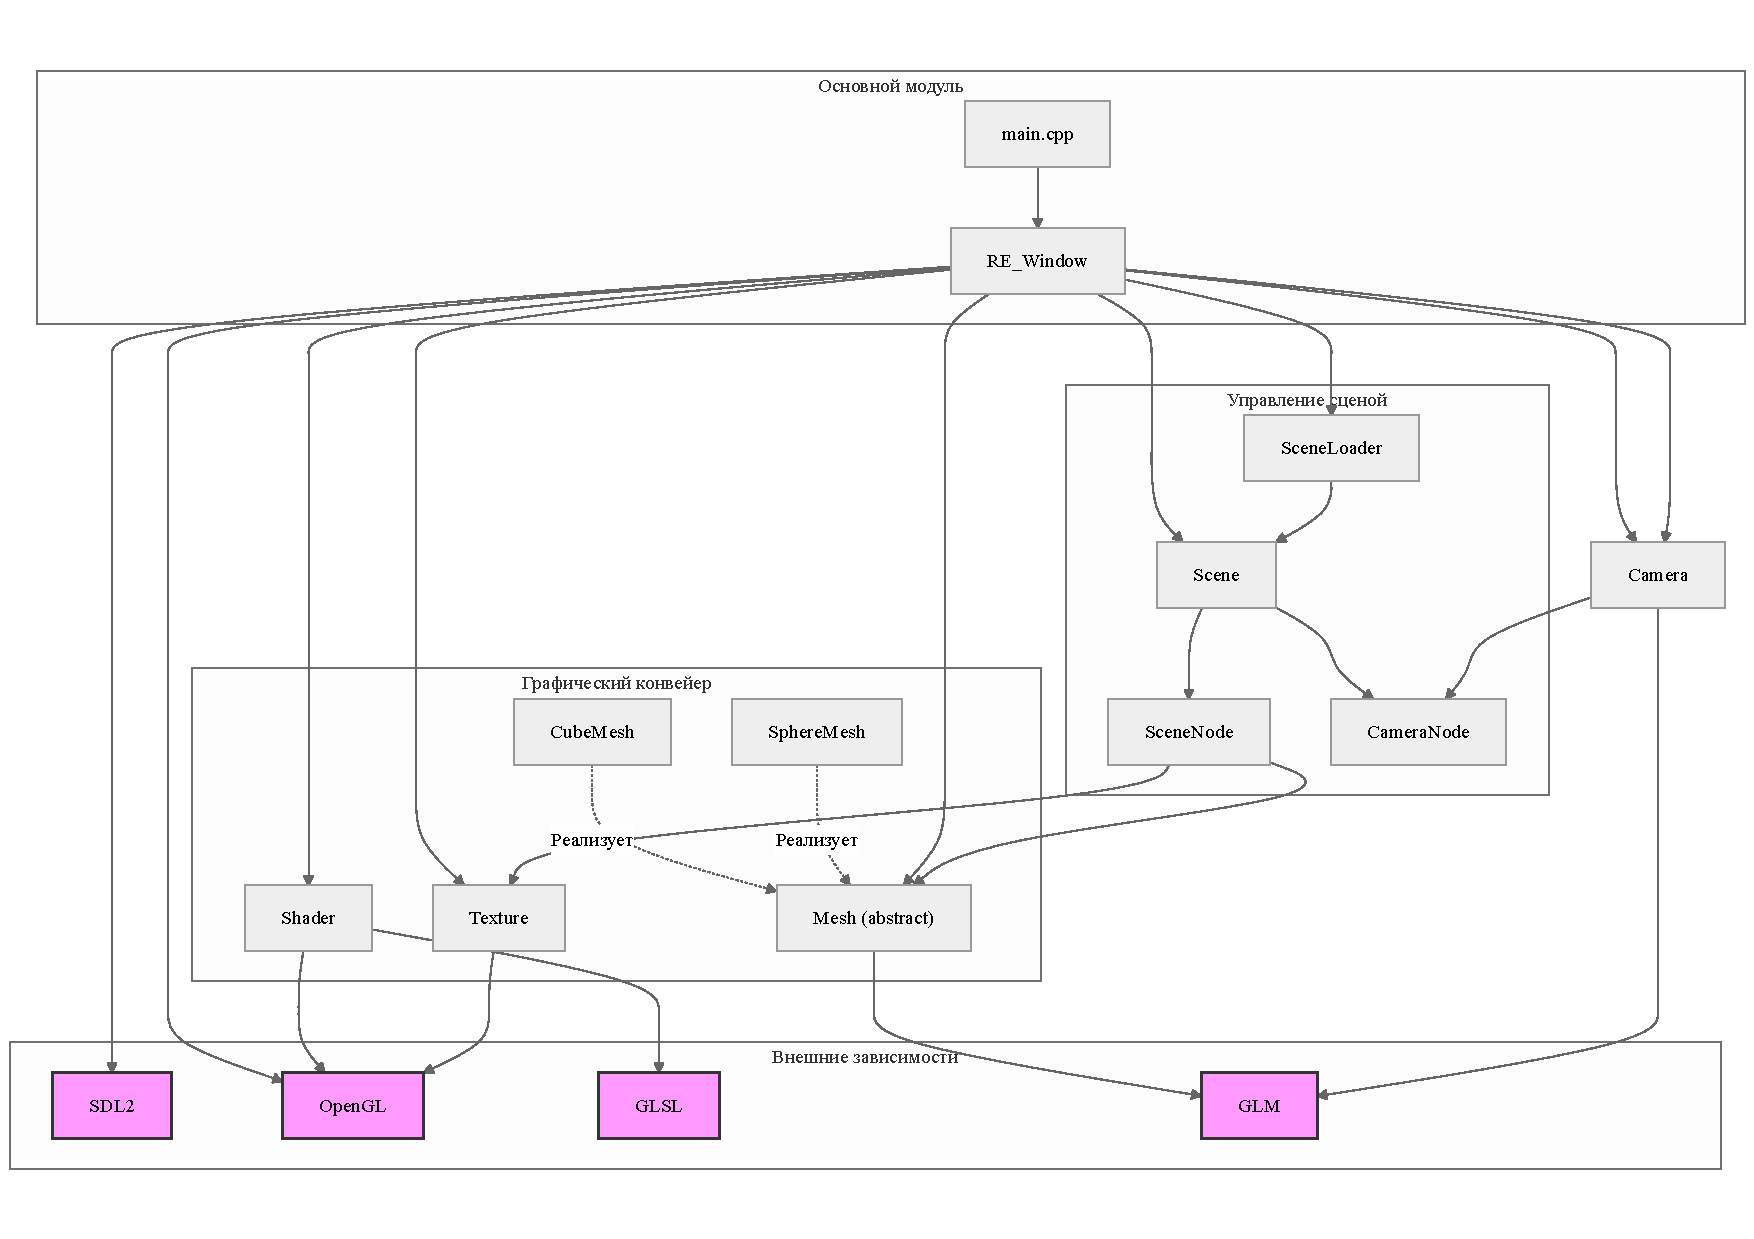
\includegraphics[width=1.6\textwidth]{comp.pdf}
      \caption{Диаграмма компонентов движка с последовательностью взаимодействия}
      \label{comp:image}
    \end{figure}
  \end{landscape}
}

\subsubsection{Состав компонентов}

Основные модули системы включают:

\begin{enumerate}
    \item Window -- компонент управления окном, реализующий:

    \begin{itemize}[itemindent=\parindent,leftmargin=\parindent]
        \item инициализацию окна;
        \item обработку ввода;
        \item обработку событий.
    \end{itemize}

    \item Renderer -- компонент управления конвейером рендеринга, реализующий абстракцию над API OpenGL. Обеспечивает:

    \begin{itemize}[itemindent=\parindent,leftmargin=\parindent]
        \item инициализацию контекста OpenGL;
        \item загрузку шейдеров;
        \item управление сценой;
        \item отрисовку сцены.
    \end{itemize}

    \item Scene -- подсистема работы со сценой:

    \begin{itemize}[itemindent=\parindent,leftmargin=\parindent]
        \item хранит коллекцию объектов (SceneNode) и управляет их состоянием;
        \item хранит камеру и параметры освещения;
        \item поддерживает цвет неба (skyColor), параметры направленного и точечных источников света (DirLight, PointLight), а также масштабируемое количество источников света.
    \end{itemize}

    \item InputHandler -- компонент обработки пользовательского ввода:

    \begin{itemize}[itemindent=\parindent,leftmargin=\parindent]
        \item предоставляет интерфейс для регистрации callback-функций на нажатие, удержание и отпускание клавиш;
        \item поддерживает обработку событий мыши (движение, нажатие, прокрутка);
        \item хранит состояния клавиш и мыши;
        \item обеспечивает получение текущей позиции и относительного перемещения мыши.
    \end{itemize}

    \item Графический конвейер (неявный компонент):

    \begin{itemize}[itemindent=\parindent,leftmargin=\parindent]
        \item Shader -- управление шейдерными программами (вершинный/фрагментный);
        \item Texture -- загрузка, генерация и привязка текстурных объектов;
        \item Mesh -- хранение геометрических данных (VBO/VAO/EBO).
    \end{itemize}

    \item Camera -- компонент управления видами, реализующий:

    \begin{itemize}[itemindent=\parindent,leftmargin=\parindent]
        \item расчёт матриц вида и проекции;
        \item преобразование координат;
        \item управление параметрами отображения (позиция, углы, FOV);
        \item относительное перемещение и вращение;
        \item получение и установка углов поворота.
    \end{itemize}
\end{enumerate}

\subsubsection{Взаимодействие компонентов}

Последовательность работы системы (рис. \ref{comp:image}) реализуется следующим образом:

\begin{enumerate}
    \item Инициализация:

    \begin{itemize}[itemindent=\parindent,leftmargin=\parindent]
        \item Renderer создаёт графический контекст;
        \item Shader компилирует шейдерные программы;
        \item SceneLoader загружает начальную сцену.
    \end{itemize}

    \item Главный цикл рендеринга:

    \begin{itemize}[itemindent=\parindent,leftmargin=\parindent]
        \item обновление матриц вида в Camera;
        \item передача uniform-переменных в шейдеры;
        \item формирование вершинного буфера объектов сцены из вектора SceneNode;
        \item отрисовка объектов сцены с учётом их:

        \begin{itemize}[itemindent=\parindent,leftmargin=\parindent]
            \item геометрии (Mesh);
            \item текстуры (Texture);
            \item шейдеров (Shader).
        \end{itemize}

        \item вывод результата через Renderer;
        \item обработка пользовательского ввода Renderer и передача его значений в Camera;
        \item повтор цикла до выхода из программы.
    \end{itemize}
\end{enumerate}

\subsection{Основные сущности системы}

Программная система состоит из сущностей, выраженных классами и структурами языка C++. Их взаимодействие реализуется через встроенные механизмы наследования и представлено в диаграмме UML (рис. \ref{uml:image}).

\afterpage{
  \begin{landscape}
    \begin{figure}[p]
      \centering
      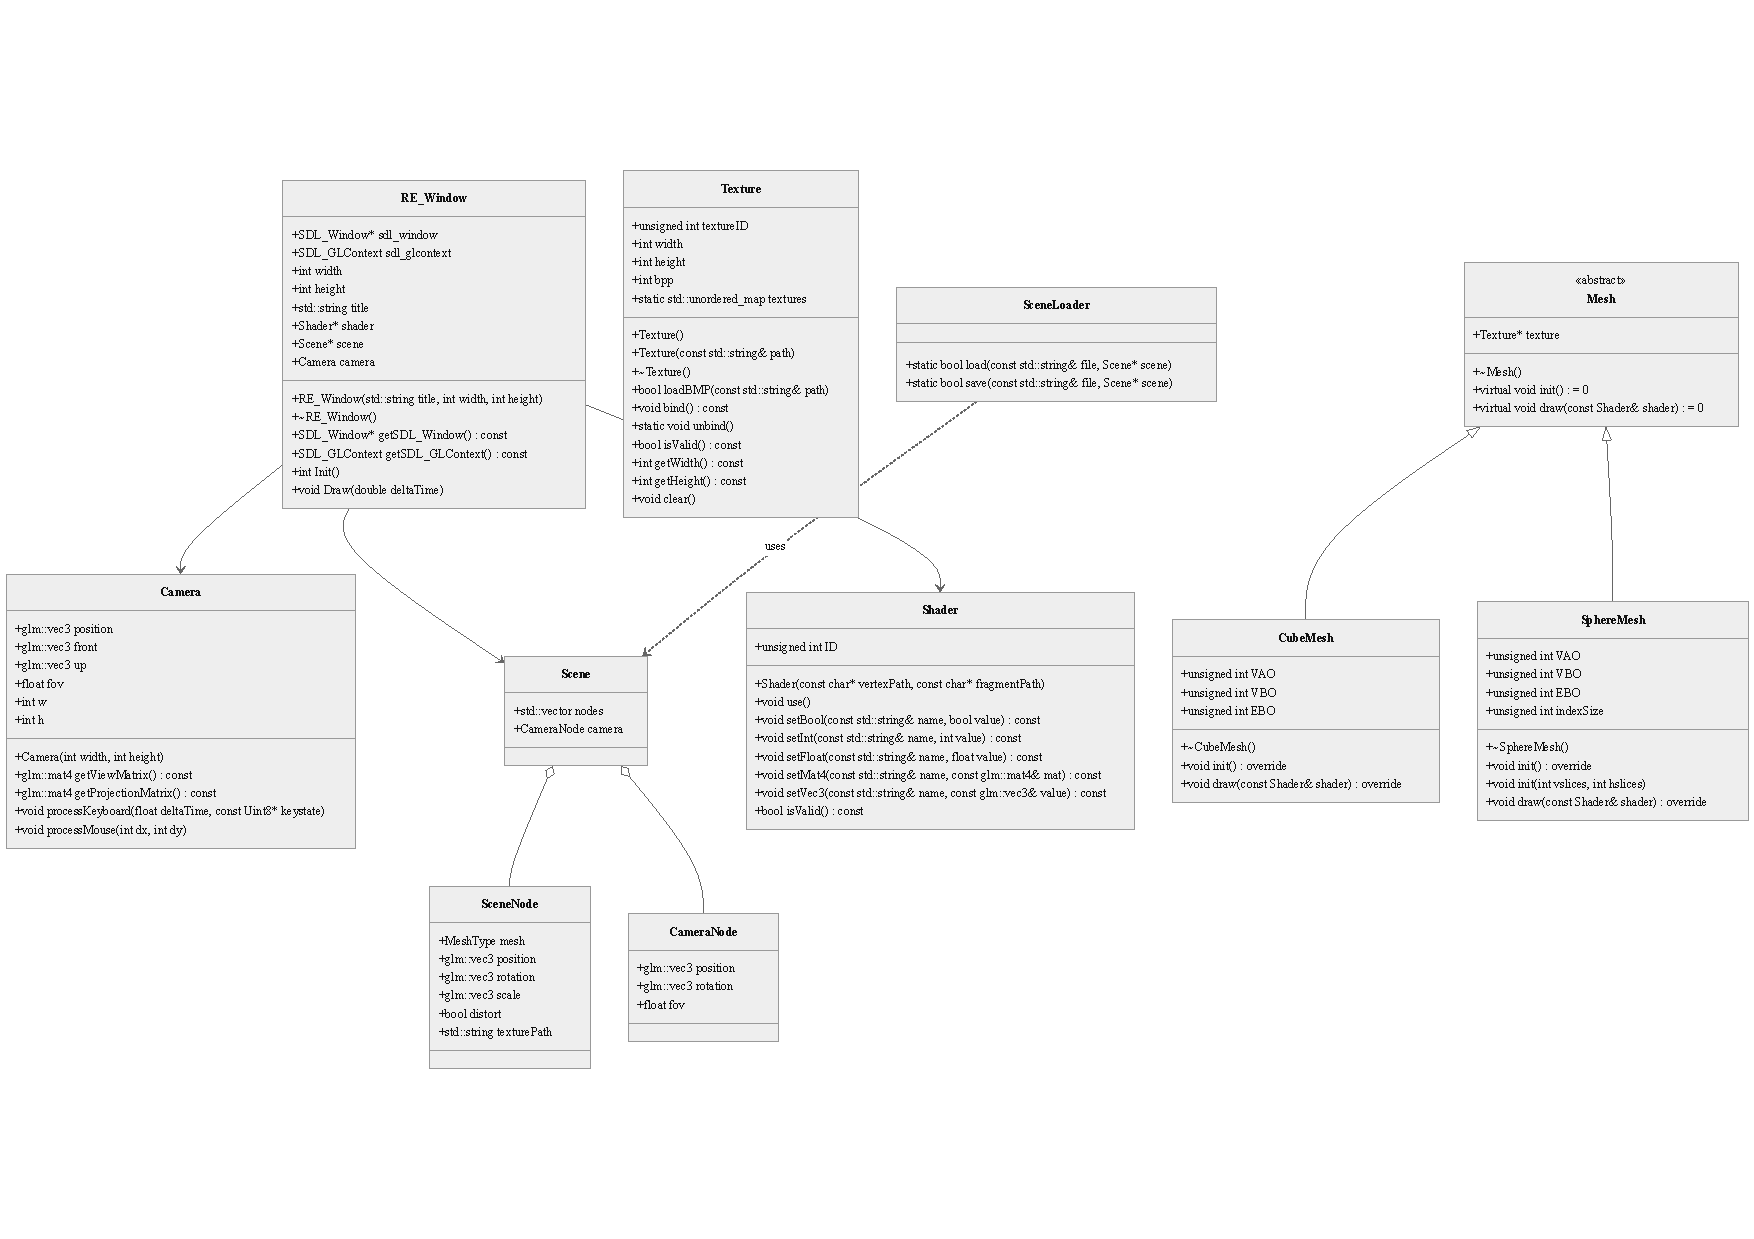
\includegraphics[width=1.6\textwidth]{uml.pdf}
      \caption{Диаграмма UML}
      \label{uml:image}
    \end{figure}
  \end{landscape}
}

\subsubsection{Класс Renderer}
Класс Renderer отвечает за управление процессом отрисовки трёхмерной сцены. Он инкапсулирует логику взаимодействия с графическим API (OpenGL), управляет объектами сцены, шейдерами и камерой. Класс не занимается напрямую созданием окна или обработкой событий, предполагая, что эти задачи решаются внешними компонентами.

Спецификация класса Renderer представлена в таблице \ref{tab:renderer_spec}.

\begin{xltabular}{\textwidth}{|X|l|X|}
    \caption{Спецификация класса Renderer\label{tab:renderer_spec}}\\ \hline
    \centrow Поле/Метод & \centrow Тип & \centrow Описание \\ \hline
    \endfirsthead
    \continuecaption{Продолжение таблицы \ref{tab:renderer_spec}}
    \centrow Поле/Метод & \centrow Тип & \centrow Описание \\ \hline 
    \finishhead

    \multicolumn{3}{|l|}{Приватные поля} \\ \hline
    width & int & Ширина области рендеринга в пикселях. \\ \hline
    height & int & Высота области рендеринга в пикселях. \\ \hline
    scene & Scene* & Указатель на объект сцены, содержащий все объекты для отображения. \\ \hline
    shader & Shader* & Указатель на объект шейдера, используемый для рендеринга объектов сцены. \\ \hline
    \multicolumn{3}{|l|}{Публичные поля} \\ \hline
    camera & Camera & Объект камеры, определяющий точку обзора и параметры проекции. \\ \hline
    \multicolumn{3}{|l|}{Методы} \\ \hline
    Renderer(int width, int height) & конструктор & Конструктор класса. Инициализирует размеры области рендеринга и камеру. \\ \hline
    getScene() & Scene* & Возвращает указатель на текущую сцену. \\ \hline
    setScene(Scene* scene) & void & Устанавливает активную сцену для рендеринга. \\ \hline
    setShader(const char* vertexPath, const char* fragmentPath) & void & Загружает и устанавливает шейдерную программу по путям к вершинному и фрагментному шейдерам. \\ \hline
    draw(unsigned long ticks) & void & Выполняет отрисовку одного кадра. ticks -- текущее время в миллисекундах. \\ \hline
\end{xltabular}

Вспомогательная функция \texttt{initRenderer(int width, int height)} (определена в \texttt{Renderer.h}) создает и возвращает указатель на новый экземпляр класса \texttt{Renderer}, инициализированный с заданной шириной и высотой.

\subsubsection{Управление окном и главный цикл}
Функциональность, связанная с созданием окна приложения, управлением главным циклом и уничтожением окна, сосредоточена в заголовочном файле \texttt{Window.h}. Этот модуль не определяет отдельный класс, а предоставляет набор функций и перечисление для кодов ошибок. Он также объявляет глобальный указатель на объект рендерера.

\paragraph{Перечисление WindowError}
Перечисление \texttt{WindowError} определяет константы для кодов ошибок, которые могут возникнуть при операциях с окном.

Спецификация перечисления WindowError представлена в таблице \ref{tab:windowerror_spec}.

\begin{xltabular}{\textwidth}{|l|X|}
    \caption{Спецификация перечисления WindowError\label{tab:windowerror_spec}}\\ \hline
    \centrow Значение & \centrow Описание \\ \hline
    \endfirsthead
    \continuecaption{Продолжение таблицы \ref{tab:windowerror_spec}}
    \centrow Значение & \centrow Описание \\ \hline 
    \finishhead
    WINDOW\_ALREADY\_EXISTS & Окно уже было создано. \\ \hline
    WINDOW\_CREATE\_FAILED & Не удалось создать окно SDL. \\ \hline
    GL\_CONTEXT\_CREATE\_FAILED & Не удалось создать контекст OpenGL. \\ \hline
    RENDERER\_INIT\_FAILED & Не удалось инициализировать рендерер. \\ \hline
\end{xltabular}

\paragraph{Функции управления окном}
Набор функций для управления жизненным циклом окна и приложения.

Спецификация функций управления окном представлена в таблице \ref{tab:windowfuncs_spec}.

\begin{xltabular}{\textwidth}{|X|l|X|}
    \caption{Спецификация функций управления окном\label{tab:windowfuncs_spec}}\\ \hline
    \centrow Функция & \centrow Возвращаемый тип & \centrow Описание \\ \hline
    \endfirsthead
    \continuecaption{Продолжение таблицы \ref{tab:windowfuncs_spec}}
    \centrow Функция & \centrow Возвращаемый тип & \centrow Описание \\ \hline 
    \finishhead
    createWindow(const char* title, int width = 0, int height = 0) & int & Инициализирует SDL, создает окно приложения и контекст OpenGL. \texttt{title} - заголовок окна. \texttt{width} и \texttt{height} - размеры окна; если 0, используется полноэкранный режим. Возвращает 0 при успехе или код ошибки из \texttt{WindowError} при неудаче. \\ \hline
    mainLoop() & void & Запускает главный цикл приложения. В цикле обрабатываются события ввода, обновляется состояние сцены и происходит отрисовка с помощью объекта \texttt{renderer}. Цикл продолжается до тех пор, пока не будет получен сигнал о закрытии окна. \\ \hline
    destroyWindow() & void & Уничтожает окно SDL, контекст OpenGL и освобождает ресурсы, связанные с рендерером и SDL. Должна вызываться перед завершением работы приложения. \\ \hline
\end{xltabular}

\subsubsection{Структура SceneNode}
Структура \texttt{SceneNode} представляет собой отдельный объект (узел) в трехмерной сцене. Она содержит информацию о геометрии объекта, его трансформациях (позиция, поворот, масштаб), материале и текстурах.

Спецификация структуры SceneNode представлена в таблице \ref{tab:scenenode_spec}.

\begin{xltabular}{\textwidth}{|l|l|X|}
    \caption{Спецификация структуры SceneNode\label{tab:scenenode_spec}}\\ \hline
    \centrow Поле & \centrow Тип & \centrow Описание \\ \hline
    \endfirsthead
    \continuecaption{Продолжение таблицы \ref{tab:scenenode_spec}}
    \centrow Поле & \centrow Тип & \centrow Описание \\ \hline 
    \finishhead
    mesh & Mesh* & Указатель на объект геометрии (меш). \\ \hline
    position & glm::vec3 & Позиция объекта в мировых координатах. Значение по умолчанию: (0,0,0). \\ \hline
    rotation & glm::vec3 & Углы поворота объекта вокруг осей X, Y, Z в градусах. Значение по умолчанию: (0,0,0). \\ \hline
    scale & glm::vec3 & Масштаб объекта по осям X, Y, Z. Значение по умолчанию: (1,1,1). \\ \hline
    shininess & float & Коэффициент блеска материала объекта. Используется в модели освещения Фонга. Значение по умолчанию: 32.0. \\ \hline
    distort & bool & Флаг, указывающий, нужно ли применять эффект искажения к текстуре объекта. Значение по умолчанию: false. \\ \hline
    texturePath & std::string & Путь к файлу основной текстуры объекта (diffuse map). \\ \hline
    specularPath & std::string & Путь к файлу текстуры для карты отражений (specular map). \\ \hline
\end{xltabular}

\subsubsection{Структура CameraNode}
Структура \texttt{CameraNode} используется для хранения конфигурации камеры в контексте сцены. Эта структура предназначена для упрощения сериализации параметров камеры при инициализации сцены. Она дублирует некоторые поля класса \texttt{Camera}, но служит для описания начального состояния камеры в сцене.

Спецификация структуры CameraNode представлена в таблице \ref{tab:cameranode_spec}.

\begin{xltabular}{\textwidth}{|l|l|X|}
    \caption{Спецификация структуры CameraNode\label{tab:cameranode_spec}}\\ \hline
    \centrow Поле & \centrow Тип & \centrow Описание \\ \hline
    \endfirsthead
    \continuecaption{Продолжение таблицы \ref{tab:cameranode_spec}}
    \centrow Поле & \centrow Тип & \centrow Описание \\ \hline 
    \finishhead
    position & glm::vec3 & Начальная позиция камеры в мировых координатах. Значение по умолчанию: (0,0,0). \\ \hline
    rotation & glm::vec3 & Начальные углы поворота камеры вокруг осей X, Y, Z в градусах. Значение по умолчанию: (0,0,0). \\ \hline
    fov & float & Угол обзора камеры (Field of View) в градусах. Значение по умолчанию: 45.0. \\ \hline
\end{xltabular}

\subsubsection{Структура DirLight}
Структура \texttt{DirLight} описывает параметры направленного источника света в сцене.

Спецификация структуры DirLight представлена в таблице \ref{tab:dirlight_spec}.

\begin{xltabular}{\textwidth}{|l|l|X|}
    \caption{Спецификация структуры DirLight\label{tab:dirlight_spec}}\\ \hline
    \centrow Поле & \centrow Тип & \centrow Описание \\ \hline
    \endfirsthead
    \continuecaption{Продолжение таблицы \ref{tab:dirlight_spec}}
    \centrow Поле & \centrow Тип & \centrow Описание \\ \hline 
    \finishhead
    direction & glm::vec3 & Вектор направления света. \\ \hline
    ambient & glm::vec3 & Интенсивность окружающего света. Компоненты (R,G,B) в диапазоне [0,1]. \\ \hline
    diffuse & glm::vec3 & Интенсивность диффузного света. Компоненты (R,G,B) в диапазоне [0,1]. \\ \hline
    specular & glm::vec3 & Интенсивность зеркального света. Компоненты (R,G,B) в диапазоне [0,1]. \\ \hline
\end{xltabular}

\subsubsection{Структура PointLight}
Структура \texttt{PointLight} описывает параметры точечного источника света. Точечный свет излучается из одной точки во всех направлениях, и его интенсивность убывает с расстоянием.

Спецификация структуры PointLight представлена в таблице \ref{tab:pointlight_spec}.

\begin{xltabular}{\textwidth}{|l|l|X|}
    \caption{Спецификация структуры PointLight\label{tab:pointlight_spec}}\\ \hline
    \centrow Поле & \centrow Тип & \centrow Описание \\ \hline
    \endfirsthead
    \continuecaption{Продолжение таблицы \ref{tab:pointlight_spec}}
    \centrow Поле & \centrow Тип & \centrow Описание \\ \hline 
    \finishhead
    position & glm::vec3 & Позиция источника света в мировых координатах. \\ \hline
    constant & float & Константный коэффициент затухания интенсивности света. \\ \hline
    linear & float & Линейный коэффициент затухания интенсивности света. \\ \hline
    quadratic & float & Квадратичный коэффициент затухания интенсивности света. \\ \hline
    ambient & glm::vec3 & Цвет окружающего света. \\ \hline
    diffuse & glm::vec3 & Цвет диффузного света. \\ \hline
    specular & glm::vec3 & Цвет зеркального света. \\ \hline
\end{xltabular}

\subsubsection{Класс Camera}
Класс Camera отвечает за управление виртуальной камерой в трехмерном пространстве. Он предоставляет методы для установки и получения позиции и ориентации камеры, вычисления матриц вида и проекции, а также для относительного перемещения и вращения. Камера использует библиотеку GLM для математических операций.

Спецификация класса Camera представлена в таблице \ref{tab:camera_spec}.

\begin{xltabular}{\textwidth}{|X|l|X|}
    \caption{Спецификация класса Camera\label{tab:camera_spec}}\\ \hline
    \centrow Поле/Метод & \centrow Тип & \centrow Описание \\ \hline
    \endfirsthead
    \continuecaption{Продолжение таблицы \ref{tab:camera_spec}}
    \centrow Поле/Метод & \centrow Тип & \centrow Описание \\ \hline 
    \finishhead

    \multicolumn{3}{|l|}{Поля} \\ \hline
    position & glm::vec3 & Позиция камеры в мировых координатах. \\ \hline
    fov & float & Угол обзора (поле зрения) камеры в градусах. \\ \hline
    w & int & Ширина окна отрисовки, используется для расчета матрицы проекции. \\ \hline
    h & int & Высота окна отрисовки, используется для расчета матрицы проекции. \\ \hline
    front & glm::vec3 & (Приватное) Вектор, указывающий направление камеры. \\ \hline
    up & glm::vec3 & (Приватное) Вектор, указывающий "верх" для камеры. \\ \hline
    \multicolumn{3}{|l|}{Методы} \\ \hline
    Camera(int width, int height) & конструктор & Конструктор. Инициализирует камеру с указанной шириной и высотой окна. \\ \hline
    setRotation(float rx, float ry, float rz) & void & Устанавливает углы поворота камеры по осям X, Y, Z (в градусах). \\ \hline
    getRotation() const & std::tuple<float, float, float> & Возвращает текущие углы поворота камеры по осям X, Y, Z (в градусах). \\ \hline
    getViewMatrix() const & glm::mat4 & Вычисляет и возвращает матрицу вида (view matrix). \\ \hline
    getProjectionMatrix() const & glm::mat4 & Вычисляет и возвращает матрицу проекции (projection matrix). \\ \hline
    moveRelative(float dx, float dy, float dz) & void & Перемещает камеру относительно ее текущей ориентации на заданные смещения. \\ \hline
    rotateRelative(float drx, float dry, float drz) & void & Поворачивает камеру относительно ее текущей ориентации на заданные углы (в градусах). \\ \hline
\end{xltabular}

\subsubsection{Структура Scene}
Структура \texttt{Scene} является контейнером для всех элементов, составляющих трехмерную сцену. Она объединяет информацию об объектах, камере, источниках света и других параметрах окружения.

Спецификация структуры Scene представлена в таблице \ref{tab:scene_spec}.

\begin{xltabular}{\textwidth}{|l|l|X|}
    \caption{Спецификация структуры Scene\label{tab:scene_spec}}\\ \hline
    \centrow Поле & \centrow Тип & \centrow Описание \\ \hline
    \endfirsthead
    \continuecaption{Продолжение таблицы \ref{tab:scene_spec}}
    \centrow Поле & \centrow Тип & \centrow Описание \\ \hline 
    \finishhead
    nodes & std::vector<SceneNode> & Список всех объектов (узлов) в сцене. \\ \hline
    camera & CameraNode & Конфигурация камеры сцены. \\ \hline
    skyColor & glm::vec3 & Цвет неба (фона) сцены. Компоненты (R,G,B) в диапазоне [0,1]. Значение по умолчанию: (0.63, 0.63, 0.85). \\ \hline
    dirLight & DirLight & Параметры направленного источника света в сцене. \\ \hline
    pointLights & std::vector<PointLight> & Список точечных источников света в сцене. \\ \hline
\end{xltabular}

\subsubsection{Перечисление MeshType}
Перечисление \texttt{MeshType} определяет типы геометрических примитивов, которые могут быть использованы в сцене:

\begin{itemize}
    \item \texttt{Cube} -- кубический примитив;
    \item \texttt{Sphere} -- сферический примитив;
    \item \texttt{Custom} -- пользовательский примитив.
\end{itemize}

\subsubsection{Абстрактный класс Mesh}
Абстрактный класс \texttt{Mesh} представляет собой базовый интерфейс для всех геометрических объектов (мешей) в сцене. Он определяет общие операции, которые должны быть реализованы всеми конкретными типами мешей, такие как отрисовка. Класс также может содержать указатели на текстуры, используемые мешем.

Спецификация класса Mesh представлена в таблице \ref{tab:mesh_spec}.

\begin{xltabular}{\textwidth}{|X|l|X|}
    \caption{Спецификация абстрактного класса Mesh\label{tab:mesh_spec}}\\ \hline
    \centrow Поле/Метод & \centrow Тип & \centrow Описание \\ \hline
    \endfirsthead
    \continuecaption{Продолжение таблицы \ref{tab:mesh_spec}}
    \centrow Поле & \centrow Тип & \centrow Описание \\ \hline 
    \finishhead
    \multicolumn{3}{|l|}{Публичные поля} \\ \hline
    texture & Texture* & Указатель на основную текстуру объекта (diffuse map). Значение по умолчанию: \texttt{nullptr}. \\ \hline
    specularTexture & Texture* & Указатель на текстуру карты отражений (specular map). Значение по умолчанию: \texttt{nullptr}. \\ \hline
    \multicolumn{3}{|l|}{Публичные методы} \\ \hline
    \textasciitilde Mesh() & виртуальный деструктор & Виртуальный деструктор для корректного освобождения ресурсов в производных классах. Реализация по умолчанию. \\ \hline
    draw(const Shader\& shader) & virtual void = 0 & Чисто виртуальный метод для отрисовки меша. Должен быть переопределен в производных классах. Принимает ссылку на используемый шейдер. \\ \hline
\end{xltabular}

\subsubsection{Класс CubeMesh}
Класс \texttt{CubeMesh} является производным от абстрактного класса \texttt{Mesh} и предназначен для создания и отрисовки стандартного трехмерного куба. Он инкапсулирует данные о вершинах, индексах и объектах буферов OpenGL, необходимых для рендеринга куба.

Спецификация класса CubeMesh представлена в таблице \ref{tab:cubemesh_spec}.

\begin{xltabular}{\textwidth}{|l|l|X|}
    \caption{Спецификация класса CubeMesh\label{tab:cubemesh_spec}}\\ \hline
    \centrow Поле/Метод & \centrow Тип & \centrow Описание \\ \hline
    \endfirsthead
    \continuecaption{Продолжение таблицы \ref{tab:cubemesh_spec}}
    \centrow Поле/Метод & \centrow Тип & \centrow Описание \\ \hline 
    \finishhead
    \multicolumn{3}{|l|}{Приватные поля} \\ \hline
    VAO & unsigned int & Идентификатор объекта вершинного массива (Vertex Array Object) OpenGL. Хранит конфигурацию атрибутов вершин. \\ \hline
    VBO & unsigned int & Идентификатор объекта вершинного буфера (Vertex Buffer Object) OpenGL. Хранит данные о вершинах куба (координаты, нормали, текстурные координаты). \\ \hline
    EBO & unsigned int & Идентификатор объекта индексного буфера (Element Buffer Object) OpenGL. Хранит индексы вершин для формирования граней куба. \\ \hline
    \multicolumn{3}{|l|}{Публичные методы} \\ \hline
    CubeMesh() & конструктор & Конструктор класса. Инициализирует буферы VAO, VBO, EBO и загружает в них данные вершин куба. \\ \hline
    \textasciitilde CubeMesh() & деструктор & Деструктор класса. Освобождает ресурсы OpenGL, связанные с VAO, VBO и EBO. \\ \hline
    draw(const Shader\& shader) & void override & Метод для отрисовки куба. Привязывает VAO, текстуры (если есть) и вызывает команду отрисовки OpenGL. Переопределяет метод базового класса \texttt{Mesh}. \\ \hline
\end{xltabular}

\subsubsection{Класс SphereMesh}
Класс \texttt{SphereMesh} является производным от абстрактного класса \texttt{Mesh} и предназначен для создания и отрисовки трехмерной сферы. Он генерирует вершины и индексы для аппроксимации сферической поверхности с заданным количеством горизонтальных и вертикальных сегментов и управляет соответствующими буферами OpenGL.

Спецификация класса SphereMesh представлена в таблице \ref{tab:spheremesh_spec}.

\begin{xltabular}{\textwidth}{|X|l|X|}
    \caption{Спецификация класса SphereMesh\label{tab:spheremesh_spec}}\\ \hline
    \centrow Поле/Метод & \centrow Тип & \centrow Описание \\ \hline
    \endfirsthead
    \continuecaption{Продолжение таблицы \ref{tab:spheremesh_spec}}
    \centrow Поле/Метод & \centrow Тип & \centrow Описание \\ \hline 
    \finishhead
    \multicolumn{3}{|l|}{Приватные поля} \\ \hline
    VAO & unsigned int & Идентификатор объекта вершинного массива (Vertex Array Object) OpenGL. \\ \hline
    VBO & unsigned int & Идентификатор объекта вершинного буфера (Vertex Buffer Object) OpenGL. Хранит данные о вершинах сферы. \\ \hline
    EBO & unsigned int & Идентификатор объекта индексного буфера (Element Buffer Object) OpenGL. Хранит индексы вершин для формирования граней сферы. \\ \hline
    indexSize & unsigned int & Количество индексов, используемых для отрисовки сферы. \\ \hline
    \multicolumn{3}{|l|}{Публичные методы} \\ \hline
    SphereMesh(int vslices = 10, int hslices = 10) & конструктор & Конструктор класса. Инициализирует буферы VAO, VBO, EBO и загружает в них данные вершин сферы, сгенерированные на основе количества вертикальных (\texttt{vslices}) и горизонтальных (\texttt{hslices}) сегментов. Значения по умолчанию: 10 для обоих параметров. \\ \hline
    \textasciitilde SphereMesh() & деструктор & Деструктор класса. Освобождает ресурсы OpenGL, связанные с VAO, VBO и EBO. \\ \hline
    draw(const Shader\& shader) & void override & Метод для отрисовки сферы. Привязывает VAO, текстуры (если есть) и вызывает команду отрисовки OpenGL. Переопределяет метод базового класса \texttt{Mesh}. \\ \hline
\end{xltabular}

\subsubsection{Класс Shader}
Класс \texttt{Shader} инкапсулирует логику загрузки, компиляции, связывания и использования шейдерных программ в OpenGL. Он позволяет загружать вершинные и фрагментные шейдеры из файлов или использовать встроенные по умолчанию, а также предоставляет удобные методы для установки uniform-переменных различных типов.

Спецификация класса Shader представлена в таблице \ref{tab:shader_spec}.

\begin{xltabular}{\textwidth}{|X|l|X|}
    \caption{Спецификация класса Shader\label{tab:shader_spec}}\\ \hline
    \centrow Поле/Метод & \centrow Тип & \centrow Описание \\ \hline
    \endfirsthead
    \continuecaption{Продолжение таблицы \ref{tab:shader_spec}}
    \centrow Поле/Метод & \centrow Тип & \centrow Описание \\ \hline 
    \finishhead
    \multicolumn{3}{|l|}{Публичные поля} \\ \hline
    ID & unsigned int & Идентификатор скомпилированной и связанной шейдерной программы OpenGL. \\ \hline
    \multicolumn{3}{|l|}{Публичные методы} \\ \hline
    Shader(const char* vertexPath = NULL, const char* fragmentPath = NULL) & конструктор & Конструктор класса. Загружает, компилирует и связывает вершинный и фрагментный шейдеры. \texttt{vertexPath} - путь к файлу вершинного шейдера, \texttt{fragmentPath} - путь к файлу фрагментного шейдера. Если пути не указаны (NULL), используются встроенные шейдеры по умолчанию. \\ \hline
    use() & void & Активирует данную шейдерную программу для использования в текущем контексте рендеринга OpenGL. \\ \hline
    setBool(const std::string \&name, bool value) const & void & Устанавливает значение uniform-переменной типа boolean в шейдере. \texttt{name} - имя переменной, \texttt{value} - значение. \\ \hline
    setInt(const std::string \&name, int value) const & void & Устанавливает значение uniform-переменной типа int в шейдере. \texttt{name} - имя переменной, \texttt{value} - значение. \\ \hline
    setFloat(const std::string \&name, float value) const & void & Устанавливает значение uniform-переменной типа float в шейдере. \texttt{name} - имя переменной, \texttt{value} - значение. \\ \hline
    setMat4(const std::string \&name, const glm::mat4 \&mat) const & void & Устанавливает значение uniform-переменной типа mat4 (матрица 4x4) в шейдере. \texttt{name} - имя переменной, \texttt{mat} - матрица. \\ \hline
    setVec3(const std::string \&name, const glm::vec3 \&value) const & void & Устанавливает значение uniform-переменной типа vec3 (вектор из 3-х компонентов) в шейдере. \texttt{name} - имя переменной, \texttt{value} - вектор. \\ \hline
    isValid() const & bool & Проверяет, была ли шейдерная программа успешно скомпилирована и связана. Возвращает \texttt{true}, если \texttt{ID != 0}, иначе \texttt{false}. \\ \hline
    \multicolumn{3}{|l|}{Приватные методы} \\ \hline
    checkCompileErrors(unsigned int shader, std::string type) & void & Вспомогательный метод для проверки ошибок компиляции или связывания шейдеров. \texttt{shader} - идентификатор объекта шейдера или программы, \texttt{type} - строка, указывающая тип проверяемого объекта ("VERTEX", "FRAGMENT" или "PROGRAM"). \\ \hline
\end{xltabular}

\subsubsection{Класс Texture}
Класс Texture предназначен для загрузки, хранения и управления текстурными данными, которые используются для наложения изображений на поверхности 3D-объектов. В текущей реализации поддерживается загрузка текстур из файлов формата BMP. Класс инкапсулирует взаимодействие с OpenGL для создания и управления текстурными объектами, а также предоставляет статический кеш для загруженных текстур, чтобы избежать повторной загрузки одних и тех же файлов.

Спецификация класса Texture представлена в таблице \ref{tab:texture_spec}.

\begin{xltabular}{\textwidth}{|X|X|X|}
    \caption{Спецификация класса Texture\label{tab:texture_spec}}\\ \hline
    \centrow Поле/Метод & \centrow Тип & \centrow Описание \\ \hline
    \endfirsthead
    \continuecaption{Продолжение таблицы \ref{tab:texture_spec}}
    \centrow Поле/Метод & \centrow Тип & \centrow Описание \\ \hline 
    \finishhead
    \multicolumn{3}{|l|}{Приватные поля} \\ \hline
    textureID & unsigned int & Идентификатор текстурного объекта OpenGL. Используется для привязки и управления текстурой в графическом конвейере. \\ \hline
    width & int & Ширина загруженной текстуры в пикселях. \\ \hline
    height & int & Высота загруженной текстуры в пикселях. \\ \hline
    bpp & int & Количество битов на пиксель в загруженной текстуре. \\ \hline
    \multicolumn{3}{|l|}{Статические публичные поля} \\ \hline
    textures & static std::unordered\_map <std::string, Texture*> & Статический ассоциативный массив (кеш) для хранения загруженных текстур. Ключом является путь к файлу текстуры. \\ \hline
    \multicolumn{3}{|l|}{Публичные методы} \\ \hline
    Texture() & конструктор & Конструктор по умолчанию. \\ \hline
    Texture(const std::string\& path) & конструктор & Конструктор, загружающий текстуру из указанного файла BMP с помощью метода \texttt{loadBMP}. \\ \hline
    \textasciitilde Texture() & деструктор & Деструктор класса. Освобождает ресурсы, связанные с текстурным объектом OpenGL, вызывая \texttt{clear()}. \\ \hline
    loadBMP(const std::string\& path) & bool & Загружает текстуру из файла формата BMP. Читает заголовки BMP, извлекает данные пикселей и вызывает \texttt{loadToGL} для загрузки в OpenGL. Возвращает \texttt{true} при успешной загрузке, иначе \texttt{false}. \\ \hline
    genFromColor(float r, float g, float b) & bool & Генерирует простую одноцветную текстуру размером 1x1 пиксель. \texttt{r, g, b} - компоненты цвета в диапазоне [0.0, 1.0]. Вызывает \texttt{loadToGL}. Возвращает \texttt{true} при успехе. \\ \hline
    bind() const & void & Привязывает текстуру (делает ее активной на текстурном юните 0) для использования в последующих операциях рендеринга. \\ \hline
    isValid() const & bool & Проверяет, была ли текстура успешно загружена и инициализирована (\texttt{textureID != 0}). \\ \hline
    getWidth() const & int & Возвращает ширину текстуры в пикселях. \\ \hline
    getHeight() const & int & Возвращает высоту текстуры в пикселях. \\ \hline
    \multicolumn{3}{|l|}{Статические публичные методы} \\ \hline
    unbind() & static void & Отвязывает текущую активную текстуру от текстурного юнита 0. \\ \hline
    \multicolumn{3}{|l|}{Приватные методы} \\ \hline
    loadToGL(std::vector <unsigned char>\& rgbData, int minFilter, int magFilter) & void & Загружает данные пикселей \texttt{rgbData} в объект текстуры OpenGL. Устанавливает параметры фильтрации (\texttt{minFilter}, \texttt{magFilter}) и режим повторения. \\ \hline
    clear() & void & Освобождает ресурсы текстурного объекта OpenGL, если он был создан (\texttt{textureID != 0}). \\ \hline
\end{xltabular}

\subsubsection{Класс InputHandler}
Класс InputHandler представляет собой статический класс, отвечающий за обработку пользовательского ввода от клавиатуры и мыши. Он использует библиотеку SDL2 для получения событий и предоставляет интерфейс для регистрации callback-функций на различные события ввода, такие как нажатие, отпускание и удержание клавиш, движение мыши, нажатие кнопок мыши и прокрутка колесика. Класс также хранит текущее состояние клавиш и позицию мыши.

Спецификация класса InputHandler представлена в таблице \ref{tab:inputhandler_spec}.

\begin{xltabular}{\textwidth}{|X|X|X|}
    \caption{Спецификация класса InputHandler\label{tab:inputhandler_spec}}\\ \hline
    \centrow Поле/Метод & \centrow Тип & \centrow Описание \\ \hline
    \endfirsthead
    \continuecaption{Продолжение таблицы \ref{tab:inputhandler_spec}}
    \centrow Поле/Метод & \centrow Тип & \centrow Описание \\ \hline 
    \finishhead

    \multicolumn{3}{|l|}{Типы данных (using)} \\ \hline
    KeyCallback & std::function<void()> & Тип для callback-функции при нажатии/отпускании клавиши. \\ \hline
    HoldKeyCallback & std::function<void(float)> & Тип для callback-функции при удержании клавиши (аргумент - deltaTime). \\ \hline
    MouseMotionCallback & std::function<void(int, int, int, int)> & Тип для callback-функции при движении мыши (x, y, xrel, yrel). \\ \hline
    MouseButtonCallback & std::function<void(int, int, int)> & Тип для callback-функции при нажатии/отпускании кнопки мыши (x, y, button). \\ \hline
    MouseWheelCallback & std::function<void(int, int)> & Тип для callback-функции при прокрутке колесика мыши (x, y смещения). \\ \hline
    \multicolumn{3}{|l|}{Статические поля (приватные)} \\ \hline
    keyStates\_ & std::unordered \_map<SDL\_Keycode, bool> & Хранит текущее состояние клавиш (нажата/отпущена). \\ \hline
    keyDownCallbacks\_ & std::unordered \_map<SDL\_Keycode, KeyCallback> & Карта callback-функций для события нажатия клавиши. \\ \hline
    keyUpCallbacks\_ & std::unordered \_map<SDL\_Keycode, KeyCallback> & Карта callback-функций для события отпускания клавиши. \\ \hline
    keyHoldCallbacks\_ & std::unordered \_map<SDL\_Keycode, HoldKeyCallback> & Карта callback-функций для события удержания клавиши. \\ \hline
    mouseButtonDown\-Callbacks\_ & std::unordered \_map<Uint8, MouseButtonCallback> & Карта callback-функций для события нажатия кнопки мыши. \\ \hline
    mouseButtonUp\-Callbacks\_ & std::unordered \_map<Uint8, MouseButtonCallback> & Карта callback-функций для события отпускания кнопки мыши. \\ \hline
    mouseMotionCallback\_ & MouseMotionCallback & Callback-функция для события движения мыши. \\ \hline
    mouseWheelCallback\_ & MouseWheelCallback & Callback-функция для события прокрутки колесика мыши. \\ \hline
    mousePosition\_ & glm::vec2 & Текущая позиция курсора мыши. \\ \hline
    mouseRelativeMotion\_ & glm::vec2 & Относительное смещение мыши с последнего кадра. \\ \hline
    \multicolumn{3}{|l|}{Статические методы} \\ \hline
    init() & static void & Инициализирует обработчик ввода. \\ \hline
    handleEvent(const SDL\_Event\& event) & static bool & Обрабатывает входящее событие SDL. Возвращает true, если событие было обработано. \\ \hline
    update(float deltaTime) & static void & Обновляет состояние ввода, вызывает callback-функции для удерживаемых клавиш. deltaTime - время с прошлого кадра. \\ \hline
    setKeyDownCallback (SDL\_Keycode key, KeyCallback callback) & static void & Устанавливает callback-функцию для события нажатия указанной клавиши. \\ \hline
    setKeyUpCallback (SDL\_Keycode key, KeyCallback callback) & static void & Устанавливает callback-функцию для события отпускания указанной клавиши. \\ \hline
    setKeyHoldCallback (SDL\_Keycode key, HoldKeyCallback callback) & static void & Устанавливает callback-функцию для события удержания указанной клавиши. \\ \hline
    setMouseMotionCallback (MouseMotionCallback callback) & static void & Устанавливает callback-функцию для события движения мыши. \\ \hline
    setMouseButtonDown\-Callback (Uint8 button, MouseButtonCallback callback) & static void & Устанавливает callback-функцию для события нажатия указанной кнопки мыши. \\ \hline
    setMouseButtonUp\-Callback (Uint8 button, MouseButtonCallback callback) & static void & Устанавливает callback-функцию для события отпускания указанной кнопки мыши. \\ \hline
    setMouseWheelCallback (MouseWheelCallback callback) & static void & Устанавливает callback-функцию для события прокрутки колесика мыши. \\ \hline
    isKeyDown (SDL\_Keycode key) & static bool & Проверяет, нажата ли указанная клавиша в данный момент. \\ \hline
    getMousePosition() & static glm::vec2 & Возвращает текущую позицию курсора мыши. \\ \hline
    getMouseRelativeMotion () & static glm::vec2 & Возвращает относительное смещение мыши с последнего кадра. \\ \hline
\end{xltabular}

\subsection{Тестирование}

Для обеспечения качества и надёжности работы информационной системы был разработан комплекс модульных тестов. Тесты включают в себя проверку корректности работы всех компонентов системы, а также тестирование различных сценариев использования.

Для разработки тестов был использован фреймворк Google Test. Он обеспечивает множество необходимых методов для написания модульных тестов, удобную интеграцию со средой разработки и системой сборки CMake.

В попытках достичь максимальной эффективности тестирования, в процессе написания тестов был использован модуль gcovr. Он позволяет оценить степень покрытия кода тестами и выявить ветви и строки, которые не затронуты тестами. По результатам анализа были созданы HTML-отчёты, визуально отображающие качество покрытия кода тестами.

Также, для выявления неоптимизированных участков кода был использован инструмент gprof, идущий в комплекте с MinGW. Он позволяет оценить время выполнения функций и выявить участки, которые необходимо заменить более оптимальными алгоритмами.
